%This work is licensed under the Creative Commons License Attribution 4.0 International (CC-BY 4.0) 
%https://creativecommons.org/licenses/by/4.0/legalcode 
\documentclass[rgb]{standalone}
\usepackage{tikz, pgfplots}
\begin{document}
	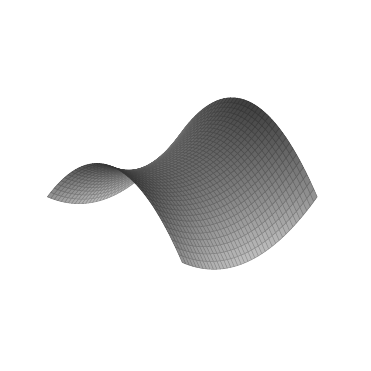
\begin{tikzpicture}[scale=0.5, font=\Large]
		\draw[draw=none] (-0.5,-1.25) -- (-0.5,6.75) -- (7.5,6.75) -- (7.5,-1.25) -- cycle;
		\begin{axis}[scale=1,clip=false,
		hide axis,
		view={45}{45},
		xmin=-2, xmax=2,
		ymin=-2, ymax=2, 
		zmin=-8, zmax=4,
		mesh/interior colormap=
		{interior}{color=(lightgray) color=(darkgray)},
		colormap=
		{exterior}{color=(lightgray) color=(darkgray)},
		samples=40,
		samples y=40,
		z buffer=sort,
		]	
		\addplot3[surf, patch, domain=-2:2, y domain=-2:2] {y^2-2*x^2};
		\end{axis}
	\end{tikzpicture}
\end{document}